% Mo Jabeen Template for docs 

\documentclass[11pt]{scrartcl} % Font size

%%%%%%%%%%%%%%%%%%%%%%%%%%%%%%%%%%%%%%%%%
% Wenneker Assignment
% Structure Specification File
% Version 2.0 (12/1/2019)
%
% This template originates from:
% http://www.LaTeXTemplates.com
%
% Authors:
% Vel (vel@LaTeXTemplates.com)
% Frits Wenneker
%
% License:
% CC BY-NC-SA 3.0 (http://creativecommons.org/licenses/by-nc-sa/3.0/)
% 
%%%%%%%%%%%%%%%%%%%%%%%%%%%%%%%%%%%%%%%%%

%----------------------------------------------------------------------------------------
%	PACKAGES AND OTHER DOCUMENT CONFIGURATIONS
%----------------------------------------------------------------------------------------

\usepackage{amsmath, amsfonts, amsthm} % Math packages

\usepackage{listings} % Code listings, with syntax highlighting

\usepackage[english]{babel} % English language hyphenation

\usepackage{graphicx} % Required for inserting images
\graphicspath{{Figures/}{./}} % Specifies where to look for included images (trailing slash required)

\usepackage{booktabs} % Required for better horizontal rules in tables

\numberwithin{equation}{section} % Number equations within sections (i.e. 1.1, 1.2, 2.1, 2.2 instead of 1, 2, 3, 4)
\numberwithin{figure}{section} % Number figures within sections (i.e. 1.1, 1.2, 2.1, 2.2 instead of 1, 2, 3, 4)
\numberwithin{table}{section} % Number tables within sections (i.e. 1.1, 1.2, 2.1, 2.2 instead of 1, 2, 3, 4)

\setlength\parindent{0pt} % Removes all indentation from paragraphs

\usepackage{enumitem} % Required for list customisation
\setlist{noitemsep} % No spacing between list items

\usepackage{array}
\newcolumntype{P}[1]{>{\centering\arraybackslash}p{#1}} %Allows centering of tables

\usepackage[
backend=biber,
style=ieee,
sorting=ynt
]{biblatex}

\addbibresource{refs.bib} %Imports bibliography file

%----------------------------------------------------------------------------------------
%	DOCUMENT MARGINS
%----------------------------------------------------------------------------------------

\usepackage{geometry} % Required for adjusting page dimensions and margins

\geometry{
	paper=a4paper, % Paper size, change to letterpaper for US letter size
	top=2.5cm, % Top margin
	bottom=3cm, % Bottom margin
	left=3cm, % Left margin
	right=3cm, % Right margin
	headheight=0.75cm, % Header height
	footskip=1.5cm, % Space from the bottom margin to the baseline of the footer
	headsep=0.75cm, % Space from the top margin to the baseline of the header
	%showframe, % Uncomment to show how the type block is set on the page
}

%----------------------------------------------------------------------------------------
%	FONTS
%----------------------------------------------------------------------------------------

\usepackage[utf8]{inputenc} % Required for inputting international characters
\usepackage[T1]{fontenc} % Use 8-bit encoding

\usepackage{fourier} % Use the Adobe Utopia font for the document

%----------------------------------------------------------------------------------------
%	HEADERS AND FOOTERS
%----------------------------------------------------------------------------------------

\usepackage{scrlayer-scrpage} % Required for customising headers and footers

\ohead*{} % Right header
\ihead*{} % Left header
\chead*{} % Centre header

\ofoot*{} % Right footer
\ifoot*{} % Left footer
\cfoot*{\pagemark} % Centre footer

%----------------------------------------------------------------------------------------
%	SECTION TITLES
%----------------------------------------------------------------------------------------
 % Include the file specifying the document structure and custom commands

%----------------------------------------------------------------------------------------
%	TITLE SECTION
%----------------------------------------------------------------------------------------


\title{	
	\normalfont\normalsize
	\vspace{20pt} % Whitespace
	{\huge Clean Architecture}\\ % The meh
	\vspace{12pt} % Whitespace
	\rule{\linewidth}{2pt}\\ % Thick bottom horizontal rule
}

\author{\small Dainish Jabeen} % Your name

\date{\normalsize\today} % Today's date (\today) or a custom date

\begin{document}

\maketitle % Print the title

Notes based on \cite{Martin17} and \cite{richards2020fundamentals}.

\tableofcontents

\pagebreak

\section{Introduction}

The goal of software architecture is to minimize the human resources
required to build and maintain the system.\\

There are two values stakeholders care about: the behavior and structure
of a system.\\

\textbf{Behavior:} Make the machine fulfill the users requirements.\\

\textbf{Architecture:} Soft ware should be easy to change, the
difficulty of the change should be proportional to the scope of change
and not the ``shape''. Shape being the type of change requested.\\

\textbf{Eisenhower matrix:} A digram showing the combination of
important and urgent. The conclusion is that generally things that are
urgent should not be important and things that are important should not
be urgent.\\

Three big areas of architecture: function, separation of components and
data management.

\section{Object orientated}

First area thought to be introduced is Encapsulation of data and
functions.\\

Data should be kept within concepts and only accessed through this
concept.\\

Good encapsulation is when the users of a program have or need no
knowledge of the implementation of the data structure or function.

\begin{itemize}
\item
  OO does not require perfect encapsulation, modern languages have
  declaration and definition of the classes tied together needing
  knowledge of one and other to use them.
\end{itemize}

\textbf{Inheritance:} Able to reuse classes and modules in different
scopes.\\

Encapsulation can exist without OO so this is not its feature.

\subsection{What is polymorphism ?}

At its core polymorphism is pointers to functions. Allowing the pointer
to dictate based on the given parameter the functions behavior.\\

This can be done without OO, however it makes it much safer and more
convenient.

\subsection{How did OO effect the flow of dependency (Dependency
inversion)}

Prior to OO (polymorphism) flow of control had to match the direction of dependency.

\begin{itemize}
\item
  All higher level functions are dependant on the implementation and the flow of
  control stems down to them from higher level function.
\end{itemize}

The dependency can be inverted using OO and interfaces; giving the
architect control over the dependency tree. \textbf{Control order does
not have to match dependency}\\

\emph{Green arrow = Control , Red arrow = dependency}

\begin{figure}[h] % [h] forces the figure to be output where it is defined in the code (it suppresses floating)
	\centering
	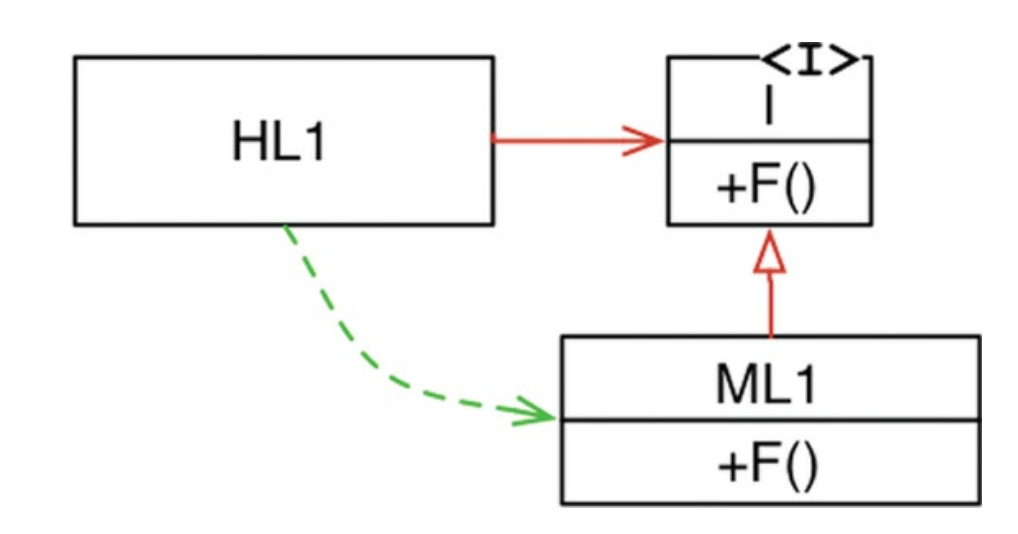
\includegraphics[width=\columnwidth]{Poly.png} % Example image
	\caption{Control/Dependency Flow}
\end{figure}

\begin{itemize}
\item
  The UI can depend on the business rules and the control flow stem from
  the rules.
\end{itemize}

\begin{figure}[h] % [h] forces the figure to be output where it is defined in the code (it suppresses floating)
	\centering
	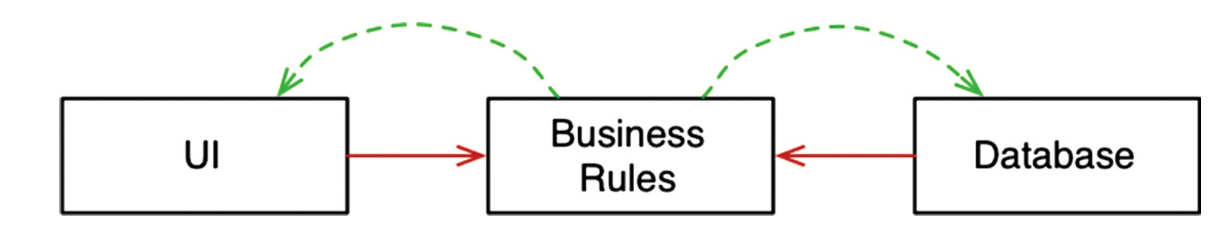
\includegraphics[width=\columnwidth]{Flow.png} % Example image
	\caption{Overview Flow}
\end{figure}

The main thing OO introduces is a safe effective method of controlling
source code dependencies !!\\

Vital to allow modularity and plugin nature of development.

\subsubsection{Functional Programming}

Functional programs variable are not mutable, they do not vary.

\textbf{All concurrent update problems derive from mutable variables}

\subsection{How do you utilize immutable variables}

If there was infinite resources (memory and processing) using immutable
variables would be an option. Instead need to split the program into
mutable and immutable components.\\

The immutable components will feed the mutable components which then use
transactional memory.\\

\begin{figure}[h] % [h] forces the figure to be output where it is defined in the code (it suppresses floating)
	\centering
	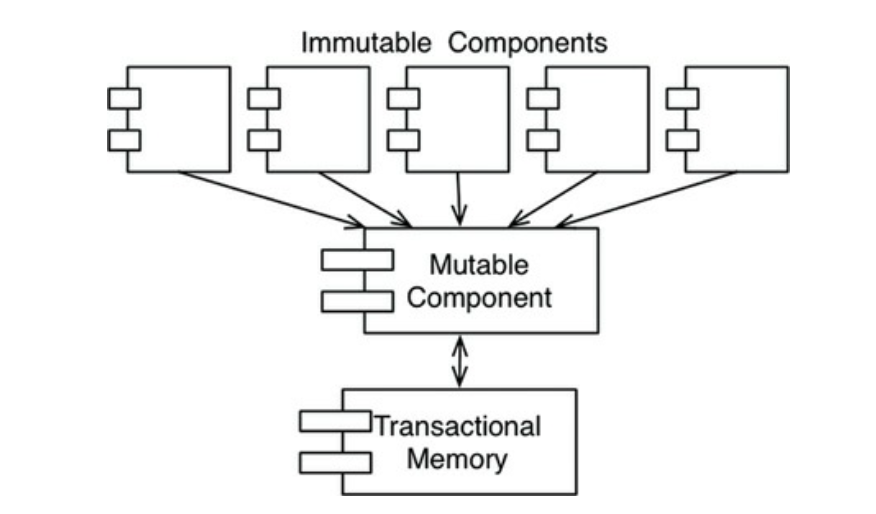
\includegraphics[width=\columnwidth]{Components.png} % Example image
	\caption{Immutable Components}
\end{figure}

Transactional memory acts as disk database with safety measures against
race conditions; locking mechanisms on reading and writing.

\subsection{What is event sourcing ?}

Store transactions instead of states to avoid mutable variables. The
state is then calculated by summing transactions.

\section{Components}

Well designed components are independently deployable and therefore
independently developable.\\

Module managment tools: Maven, Leiningen and RVM.\\

Three principles associated with component design :

\subsection{Reuse/Release equivalence principle}

Should be an overarching theme of the modules inside a component.\\

To allow effective developing and reuse of a component there should be
scheduled releases of new versions. And therefore the classes and
components should be releasable together as a unit.

\subsection{Common closure principle}

Gather classes/modules into a component that change for the same
reasons at the same time.\\

Much easier to change related classes in a single component than across
many components.

\subsection{Common reuse principle}

Dont force users of a component to depend on code they dont need.
Place reused classes and modules together into a component. There
should be a high dependency in a component's classes and modules.\\

If dependant on a component better to be completely dependant on the
entire component.

\subsection{How do you balance the three principles}

It is dependant on the needs of the software system and there will be
tension between all three.\\

i.e Early on development CCP is more important than REP ! As development
is more important than reuse.

\begin{figure}[h] % [h] forces the figure to be output where it is defined in the code (it suppresses floating)
	\centering
	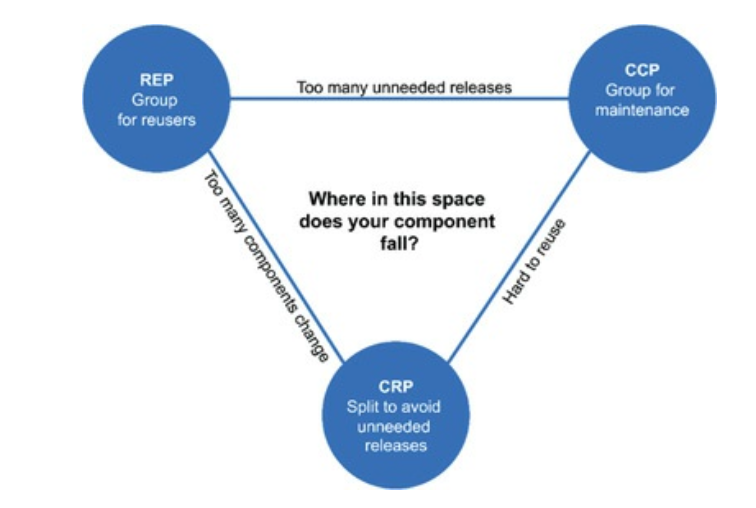
\includegraphics[width=\columnwidth]{space.png} % Example image
	\caption{Balancing three principles}
\end{figure}

\section{Component Cohesion}

\subsection{Acyclic dependencies principle}

No cycles in the component dependency graph.\\

Released components allow devs to work in isolated teams and decide
which version to integrate with their dependant component.\\

If there is a dependency cycle between components multiple components
will be forced to use the same version of a dependant components
disrupting the isolated teams.\\

To break a cycle create an interface component which will inverse the
dependency. Or create another component between.

\subsection{Stable dependency principle}

Do not make hard to change modules depend on easy to change modules.\\

A method to make software stable and therefore hard to change is to have
a lot of software dependant on it.

\subsubsection{How do you measure stability ?}

By the number of dependencies:\\

Fan in: Incoming dependencies (Increasing this number is good for
stability) Fan out: Outgoing dependencies\\

Instability : I = Fan out/(Fan in + Fan out), I=0 is maximum stability
and I=1 is max unstable.

\subsection{Stable abstraction principle}

A component should be as abstract as it is stable.\\

A stable component should be abstracted so it can be \textbf{extended},
it should be hard to change however being extendable does not effect
this.

\subsubsection{How can you measure abstractness}

Abstractness = Number of abstract classes and interfaces / number of
classes in component

\begin{figure}[h] % [h] forces the figure to be output where it is defined in the code (it suppresses floating)
	\centering
	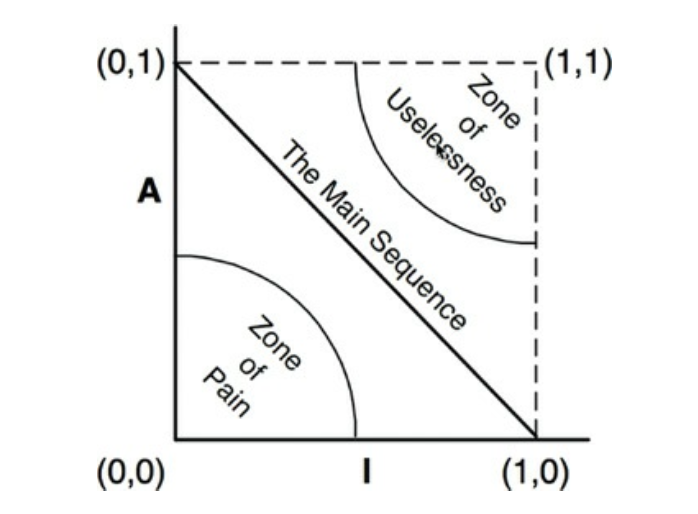
\includegraphics[width=\columnwidth]{main_seq.png} % Example image
	\caption{Abstractness measurement}
\end{figure}

\subsubsection{Metric to determine good design}

Distance from main sequence :

D = \textbar{} A + I -1 \textbar{}

\section{Architecture}

Architecture is about deployment, maintenance and ongoing development.
Not directly linked with behavior or operation however it can aid in
this.\\

The focus is on reliability and development speed not performance. Good architecture is about
making a system easy to understand, develop, deploy and maintain.\\

As many options as possible should be kept open for as long as possible
by good design. Until you are in the most optimum position to make a
judgment on an option (database, language, hardware etc).\\

The concept is to ensure policy is completely decoupled from details.\\

Good architecture is about balancing when boundaries are needed and not needed and being flexible 
about this as it will be revealed as time progresses. Trade offs are always present.

\subsection{Technical Breadth}

All architecture will be iterative due to unknown unknown, the response is to reduce this by increasing
your known unknowns - technical breadth.\\

Careful to avoid the frozen caveman problem, constantly revisiting the same risk due to PTSD.

\subsection{Areas}

Software architecture can be thought of as involving work in four paradigms.

\begin{itemize}
  \item Structure: Deployment method (Monolithic,Distributed)
  \item Characteristics: Properties to focus on based on domain problem (Performance,Security,Scalability)
  \item Decisions: Hard rules for constructing the system (only procedures can access the database)
  \item Principles: Soft rules/guidance (Only use asynchronous comms)
\end{itemize}

\subsection{Characteristics}

The list of characteristics supported should be as small as possible for simplicity.

\begin{table}
  \centering
  \begin{tabular}{|c|p{8cm}|}
    \hline
    \textbf{Metric} & \textbf{Definition} \\ \hline
    \textbf{Availability} & How long the system will need to be available (if 24/7, steps need to be in place to allow the system to be up and running quickly in case of any failure). \\ \hline
    \textbf{Performance} & Includes stress testing, peak analysis, analysis of the frequency of functions used, capacity required, and response times. Performance acceptance sometimes requires an exercise of its own, taking months to complete. \\ \hline
    \textbf{Reliability/safety} & Assess if the system needs to be fail-safe, or if it is mission critical in a way that affects lives. If it fails, will it cost the company large sums of money? \\ \hline
    \textbf{Scalability} & Ability for the system to perform and operate as the number of users or requests increases. \\ \hline
  \end{tabular}
  \caption{Operational Characteristics}
\end{table}

\begin{table}
  \centering
  \begin{tabular}{|c|p{8cm}|}
    \hline
    \textbf{Metric} & \textbf{Definition} \\ \hline
    \textbf{Configurability} & Ability for the end users to easily change aspects of the software’s configuration (through usable interfaces). \\ \hline
    \textbf{Extensibility} & How important it is to plug new pieces of functionality in. \\ \hline
    \textbf{Installability} & Ease of system installation on all necessary platforms. \\ \hline
    \textbf{Localization} & Support for multiple languages on entry/query screens in data fields; on reports, multibyte character requirements and units of measure or currencies. \\ \hline
    \textbf{Portability} & Does the system need to run on more than one platform? (For example, does the frontend need to run against Oracle as well as SAP DB?) \\ \hline
    \textbf{Upgradeability} & Ability to easily/quickly upgrade from a previous version of this application/solution to a newer version on servers and clients. \\ \hline
    \textbf{Leverageability/reuse} & Ability to leverage common components across multiple products. \\ \hline
    \textbf{Maintainability} & How easy it is to apply changes and enhance the system? \\ \hline
    \textbf{Supportability} & What level of technical support is needed by the application? What level of logging and other facilities are required to debug errors in the system? \\ \hline
    \end{tabular}
    \caption{Structural Characteristics}
\end{table}

\begin{table}
  \centering
  \begin{tabular}{|c|p{8cm}|}
    \hline
    \textbf{Metric} & \textbf{Definition} \\ \hline
    \textbf{Accessibility} & Access to all your users, including those with disabilities like colorblindness or hearing loss. \\ \hline
    \textbf{Archivability} & Will the data need to be archived or deleted after a period of time? (For example, customer accounts are to be deleted after three months or marked as obsolete and archived to a secondary database for future access.) \\ \hline
    \textbf{Authentication} & Security requirements to ensure users are who they say they are. \\ \hline
    \textbf{Legal} & What legislative constraints is the system operating in (data protection, Sarbanes Oxley, GDPR, etc.)? What reservation rights does the company require? Any regulations regarding the way the application is to be built or deployed? \\ \hline
    \textbf{Security} & Does the data need to be encrypted in the database? Encrypted for network communication between internal systems? What type of authentication needs to be in place for remote user access? \\ \hline
    \textbf{Usability/achievability} & Level of training required for users to achieve their goals with the application/solution. Usability requirements need to be treated as seriously as any other architectural issue. \\ \hline
    \textbf{Authorization} & Security requirements to ensure users can access only certain functions within the application (by use case, subsystem, webpage, business rule, field level, etc.). \\ \hline
    \textbf{Privacy} & Ability to hide transactions from internal company employees (encrypted transactions so even DBAs and network architects cannot see them). \\ \hline
    \textbf{Supportability} & What level of technical support is needed by the application? What level of logging and other facilities are required to debug errors in the system? \\ \hline
    \end{tabular}
    \caption{Cross cutting characteristics}
\end{table}

\subsubsection{Domain}

\begin{table}
  \centering
  \begin{tabular}{|c|p{6cm}|p{6cm}|}
    \hline
    \textbf{Domain concern} & \textbf{Architecture characteristics} & \textbf{Example} \\ \hline
    \textbf{Mergers and acquisitions} & Interoperability, scalability, adaptability, extensibility & The system needs to be able to integrate with the systems of the acquired company and scale to meet the needs of the larger organization. \\ \hline
    \textbf{User satisfaction} & Performance, availability, fault tolerance, testability, deployability, agility, security & The system needs to be responsive, always available, and secure in order to meet the needs of users. \\ \hline
    \textbf{Time and budget} & Simplicity, feasibility & The system needs to be easy to develop and maintain within the constraints of time and budget. \\ \hline
    \textbf{Time to market} & Agility, testability, deployability & The system needs to be developed and deployed quickly in order to meet market demands. \\ \hline
    \textbf{Competitive advantage} & Agility, testability, deployability, scalability, availability, fault tolerance & The system needs to be able to adapt to changing market conditions and provide a competitive advantage for the organization. \\ \hline
    \end{tabular}
    \caption{Mapping from domain to characteristics}
\end{table}

\subsection{Size}

The needs for different sized groups will be different. Small groups may find many interfaces and 
complete modularization a hindrance. A component per team may not be the optimal method of balancing
deployment, operation and maintenance even if it makes development easier.\\

I.e Following strict micro service method will add heavier interconnections burden and bottleneck 
deployment, even if it helps development via strong boundaries. Immediate deployment should
always be the goal.

\subsection{Maintenance}

The primary maintenance cost is splunking; finding the best place in software to add a feature or repair.
With the risk of changes causing unwanted bugs. Clean architecture should via screaming its use cases and strong
boundaries limit this.

\subsection{Use Cases}

The use case should be made clear by the architecture, behavior/features are easy to find via
prominent modules.\\

Many human resources have been wasted by decisions made on the details not relevant to the use case.
These should be deffered as long as possible. 

\subsection{Diagrams}

Good to simplfy diagrams by only showing interface points and using splits to show 
different data flow streams.

\section{Dependency}

Dependency can be thought of as import mechanisms, if a module or files requires an import or using
statement then it is \textbf{dependant on the thing its is importing!}\\

\textbf{Connascense:} Change in one module requires change in another to keep the system working.

An interface allows for dependency inversion without changing the flow of control. This is vital
to a modularized methodology. The key thing to check in dependency is if changes or breakages
 in a module effect other modules, if they do they are dependant.\\

Generally an interface is called via a data object allowing for polymorphic methods and independence.\\

\begin{figure}[h] % [h] forces the figure to be output where it is defined in the code (it suppresses floating)
	\centering
	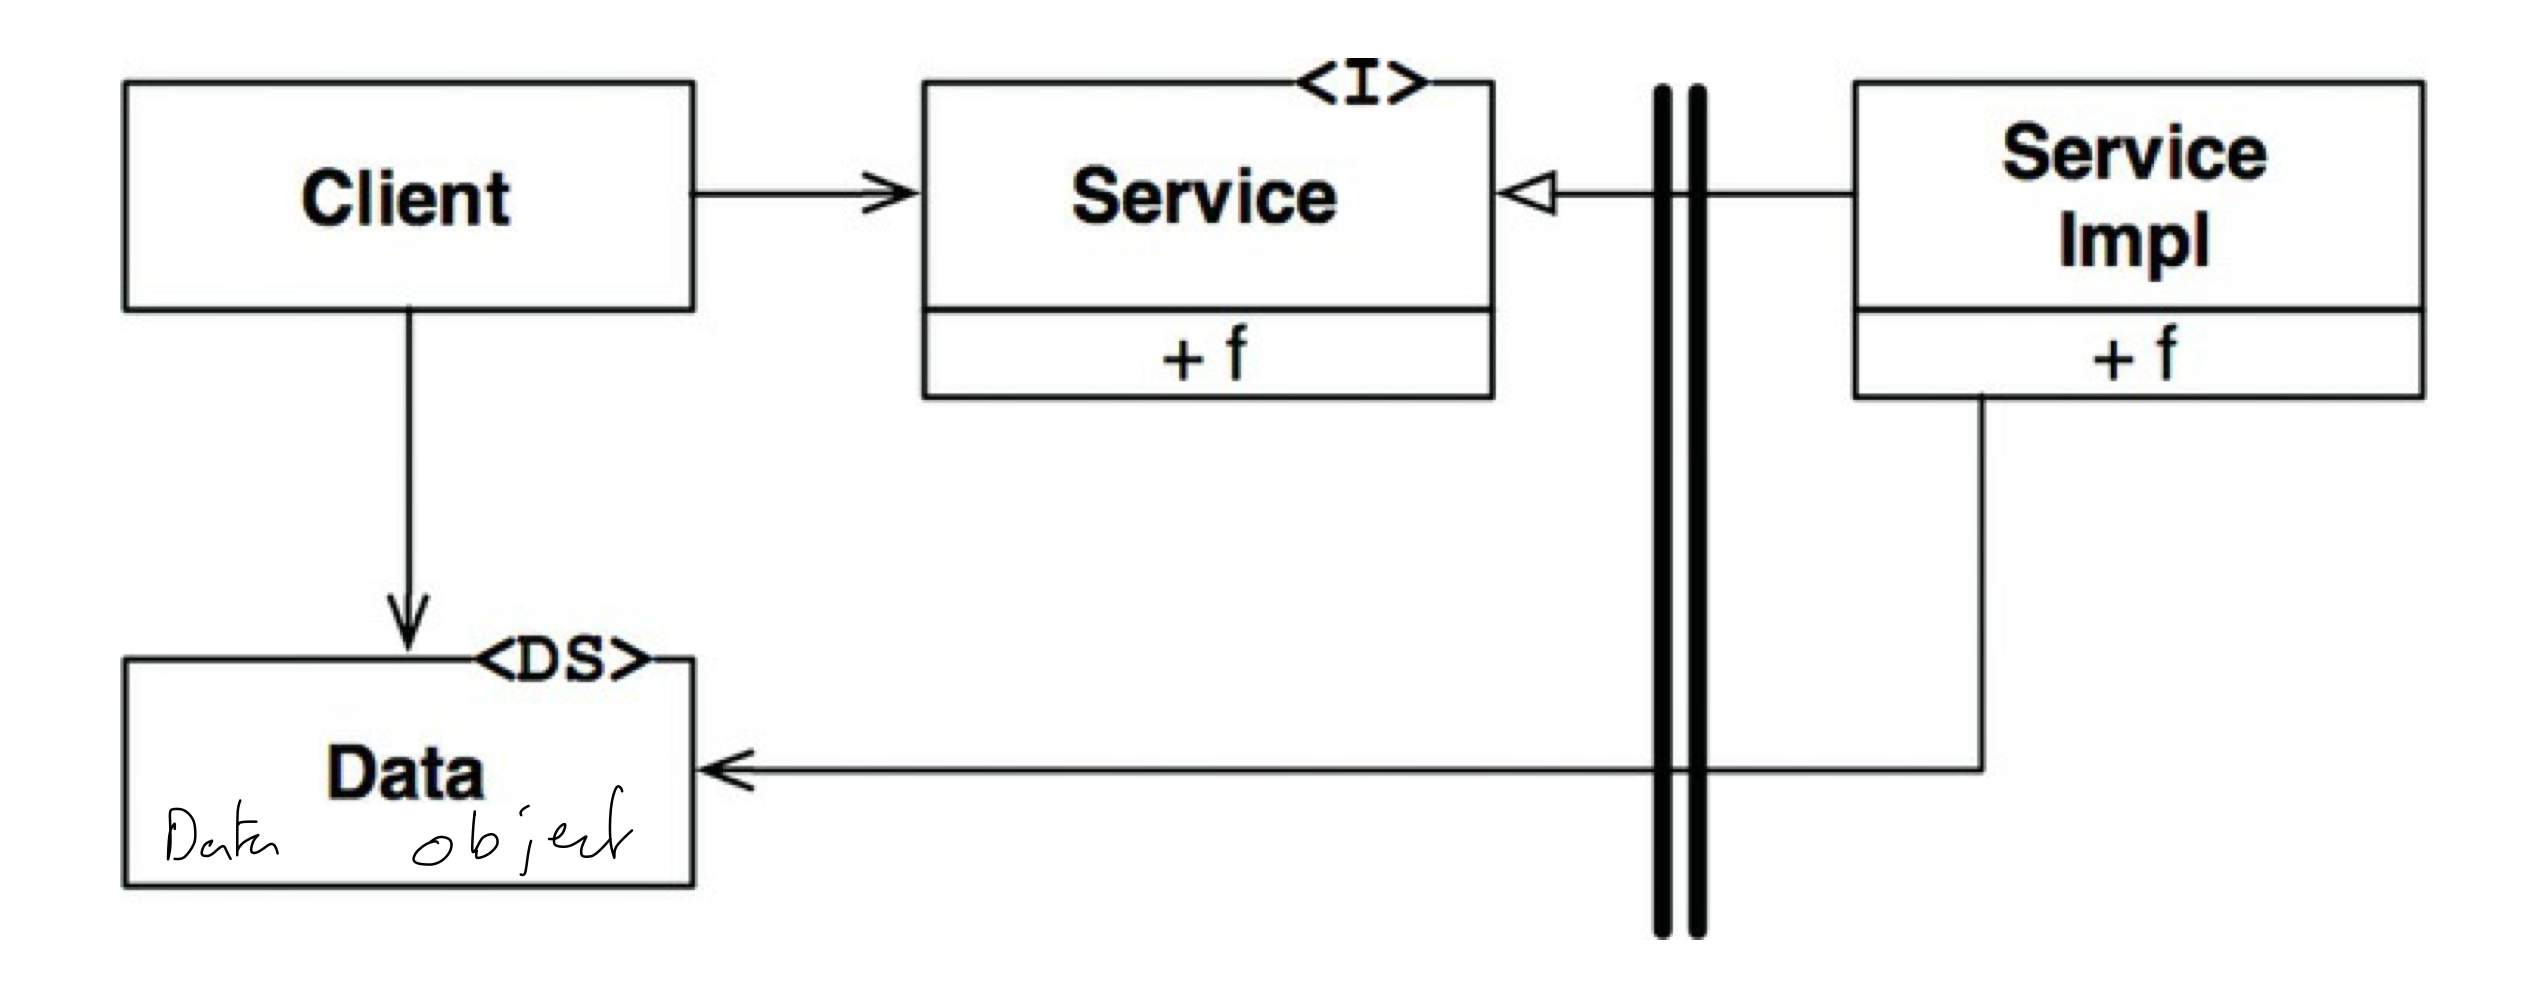
\includegraphics[width=\columnwidth]{Interface.jpeg} % Example image
	\caption{Interfaces boundaries}
\end{figure}

The lower level component should depend on the higher level ones. I.e DB access method should depend 
on the procedure that uses that data and not the other way. This allows for plugin design where details
are dependant on procedures so they can be easily swapped.\\

\textbf{Vital to remember to create reusable interfaces/frameworks, must create them concurrently with several plugins/reusing apps.}\\

Error handling becomes clear when there is clear dependency as it can happen post interface.

\section{Component Cohesion}

A module should be determined by the axis of changes, is it expected for all elements
in this module to change for the same reason and rate!\\

A module hard to change should be easy to extend.

\section{Decoupling}

Separate things that change for different reasons collect things that change for the same reason.
(UI and procedures change for different reasons). All implementation details should change for 
different reasons than core procedures and therefore should be independent.\\

Technical elements are the horizontal layers, and use cases/actors are the vertical layers. A use 
case may need many technical elements across the layers (UI,procedure and DB).\\

This may cause duplication, however if this will eventually diverge (accidental duplication) it is 
acceptable.\\

The data passing between boundaries should not have structure that causes dependencies, as this will
cause dependency inversion to be broken. It should be kept as simple as possible and then formatted
after the boundary.\\

To determine coupling determine if any new features require coordination between components.

\subsection{Methods}

\begin{itemize}
  \item Source code level: Monolithic structure, comms via functions calls
  \item Deployment level: Individually deployed units, comms via sockets or shared mem.
  \item Service level: Independent at source level, comms via network
\end{itemize}

Tip: Best to keep modules ready for separation as services, however not to separate unless good reason.

\section{Policies}

Policies lead to procedures and should be separated and grouped together based on axis of change.
The grouped policies are components on acyclic graph.

\begin{lstlisting}[
	caption= Bad design, % Caption above the listing
	language=python, % Use Julia functions/syntax highlighting
	frame=single, % Frame around the code listing
	showstringspaces=false, % Don't put marks in string spaces
	numbers=left, % Line numbers on left
	numberstyle=\large, % Line numbers styling
	]

	func encrypt() {
    while(true)
      writeChar(translate(readChar()))
  }

\end{lstlisting}

This is bad design as the procedure encrypt is dependant on the details. \\

\begin{figure}[h] % [h] forces the figure to be output where it is defined in the code (it suppresses floating)
	\centering
	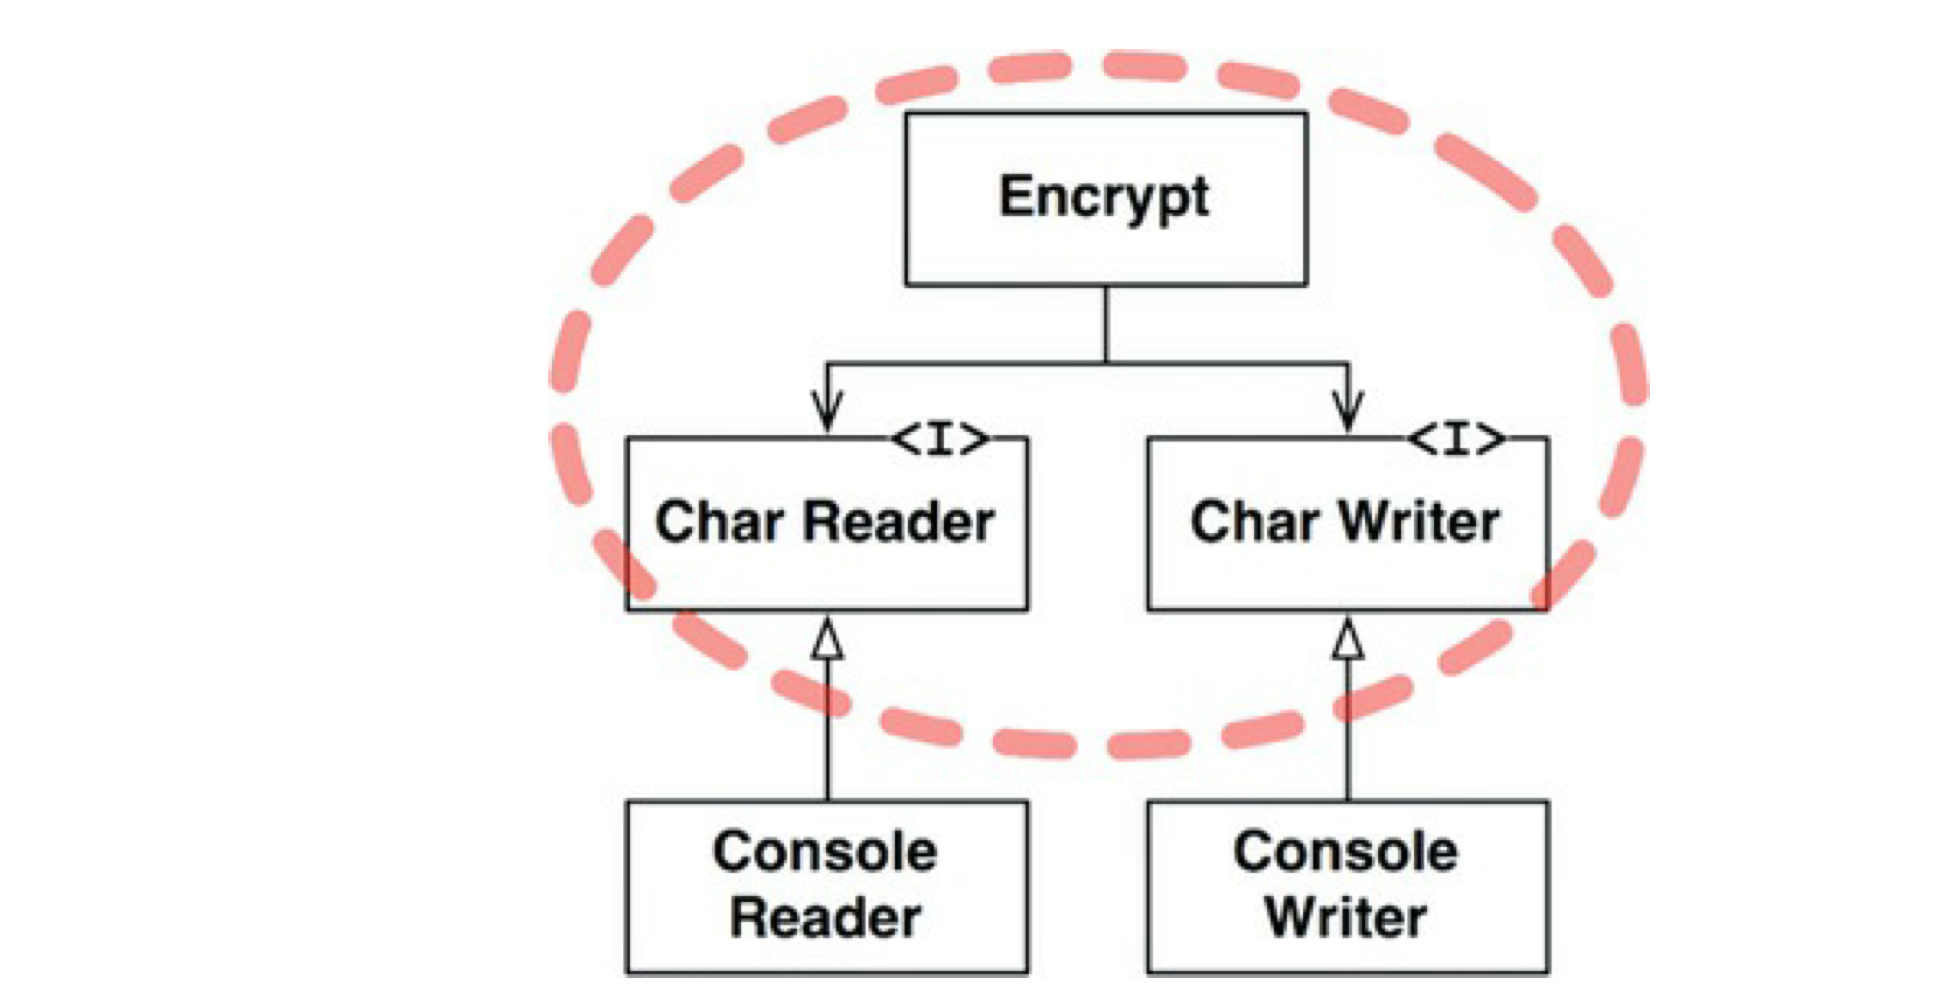
\includegraphics[width=\columnwidth]{Improved.jpeg} % Example image
	\caption{Improved Architecture}
  \label{Improved}
\end{figure}

A better design would be: Figure \ref{Improved}.

\subsection{Critical}

The highest level procedures should be those that could be done manually, at the core of product.
These can be considered critical procedures.

\section{Partial Boundaries}

If a full boundary might be needed in the future.

Facade classes are stand in place methods that don't have dependency inversion to access services.

\section{Testing}

\textbf{Humble object pattern:} Separate easy to test presenter and hard to test view.\\

The view is the detail hardware and the presenter is the methods used to get the data to it. The view
module should be kept very simple to allow the rest of the code to be easily tested.\\

Interfaces allow views/controllers to be replaced with stubs or test doubles easily.\\

\textbf{Fragile tests:} Strong coupling between tests and code mean changes in the code cause all tests to break.\\

\textbf{Create a test API to access the procedures, decoupling the structure of the tests and procedures.}

\section{Main component}

This should oversee and coordinate everything, it is the lowest level policy. Nothing should be
dependant on it, other than the operating system.\\

Main should setup initial conditions and configurations and hand this over to higher level policies.
If designed as a plugin allows many different configurations.

\section{Services}

Services that don't follow the dependency inversion rule (using interfaces) are not architecturally significant,
despite being computationally separate they maybe coupled via the data shared. If a change to the shared data
causes many services to need change.\\

Each service should have its own boundaries dividing it into components, the real boundaries are not between the
services they are interfaces communicating with each other. Unless the service is a single component surrounded by boundaries.\\

The benefit of service design is outside the goal of good architecture.

\section{Structures}

\begin{itemize}
  \item Big ball of mud: None
  \item Monolithic
  \begin{itemize}
    \item Layered
    \item Pipeline
    \item Microkernal
  \end{itemize}
  \item Distributed
  \begin{itemize}
    \item Service-based
    \item Event driven
    \item Space based
    \item Service-orientated
    \item Microservices
  \end{itemize}
\end{itemize}

Distributed gives the benefit of performance,scalability and availability with a bunch of networking headaches.

\subsection{Layered}

Separated components based on technical differences.\\

\begin{figure}[h] % [h] forces the figure to be output where it is defined in the code (it suppresses floating)
	\centering
	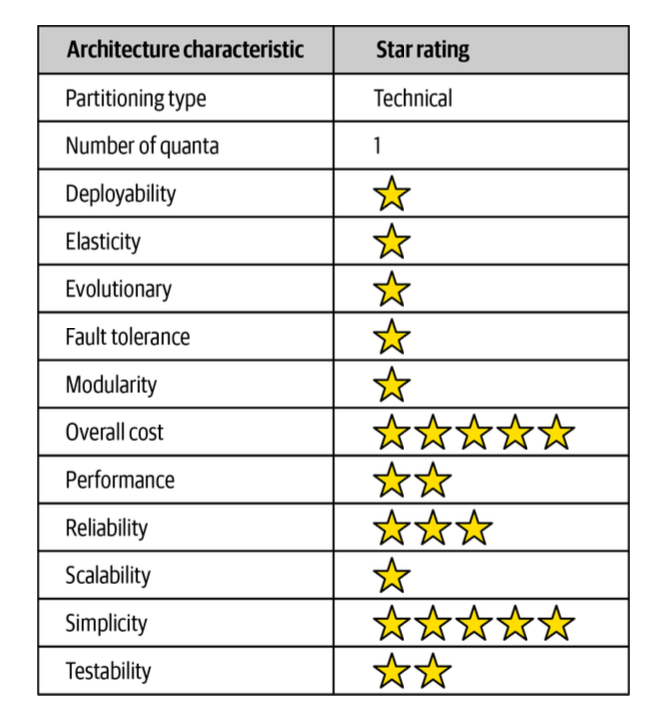
\includegraphics[width=\columnwidth]{Layered.png} % Example image
	\caption{Layered Rating}
  \label{Layered}
\end{figure}

Rating table found in Figure:\ref{Layered} on page: \pageref{Layered}.

\subsection{Pipeline}

Filter and pipe method, where data is passed through many stateless filters via pipes.\\

\begin{figure}[h] % [h] forces the figure to be output where it is defined in the code (it suppresses floating)
	\centering
	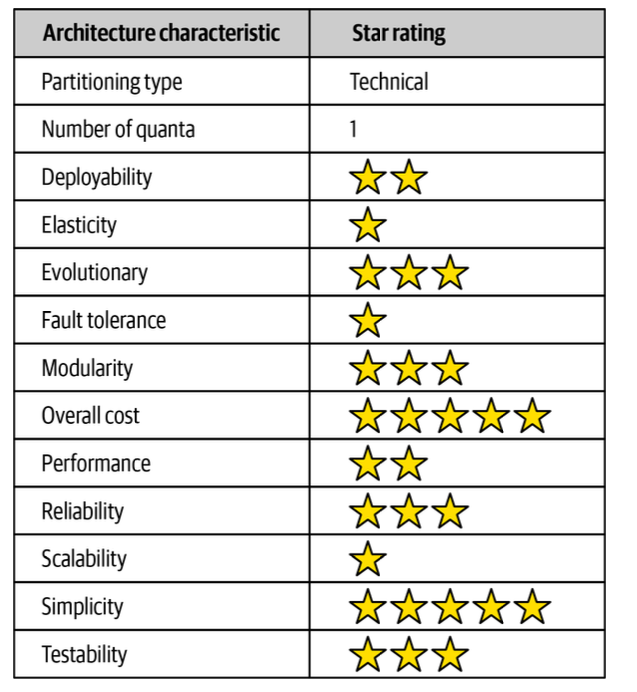
\includegraphics[width=\columnwidth]{Pipeline.png} % Example image
	\caption{Pipeline Rating}
  \label{Pipeline}
\end{figure}

Rating table found in Figure:\ref{Pipeline} on page: \pageref{Pipeline}.

\subsection{Microkernal}

Division of components by technical and domain. Gives plugin structure.\\

\begin{figure}[h] % [h] forces the figure to be output where it is defined in the code (it suppresses floating)
	\centering
	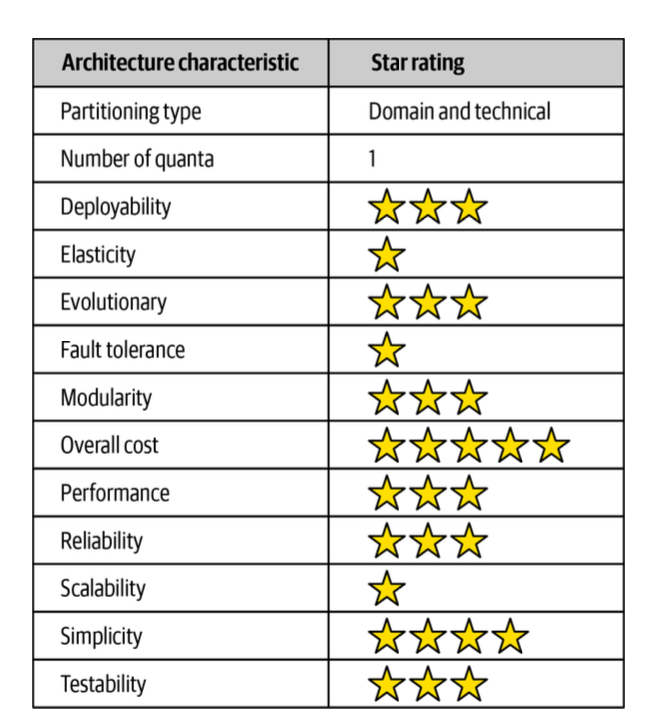
\includegraphics[width=\columnwidth]{Microkernal.png} % Example image
	\caption{Microkernal Rating}
  \label{Microkernal}
\end{figure}

Rating table found in Figure:\ref{Microkernal} on page: \pageref{Microkernal}.

\subsection{Service-based}

The basic topology of service-based architecture follows a distributed macro layered
structure consisting of a separately deployed user interface, separately 
deployed remote coarse- grained services, and a monolithic database. The services split by domain.\\

\begin{figure}[h] % [h] forces the figure to be output where it is defined in the code (it suppresses floating)
	\centering
	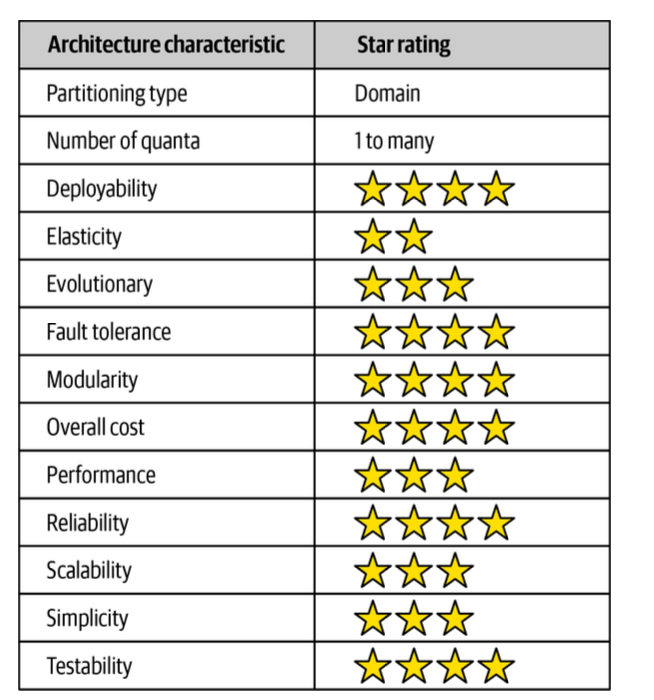
\includegraphics[width=\columnwidth]{Service-based.png} % Example image
	\caption{Service based Rating}
  \label{Service-based}
\end{figure}

Rating table found in Figure:\ref{Service-based} on page: \pageref{Service-based}. 

\subsection{Event-driven}

Event-driven architecture is made up of decoupled event processing components that asynchronously 
receive and process events. It can be used as a standalone architecture 
style or embedded within other architecture styles (such as an event-driven microservices architecture).\\

Requests made to the system to perform some sort of action are send to a request orchestrator.
The request orchestrator is to deterministically and synchronously direct the request to various 
request processors. The request processors handle the request, either retrieving or updating 
information in a database.\\

\begin{figure}[h] % [h] forces the figure to be output where it is defined in the code (it suppresses floating)
	\centering
	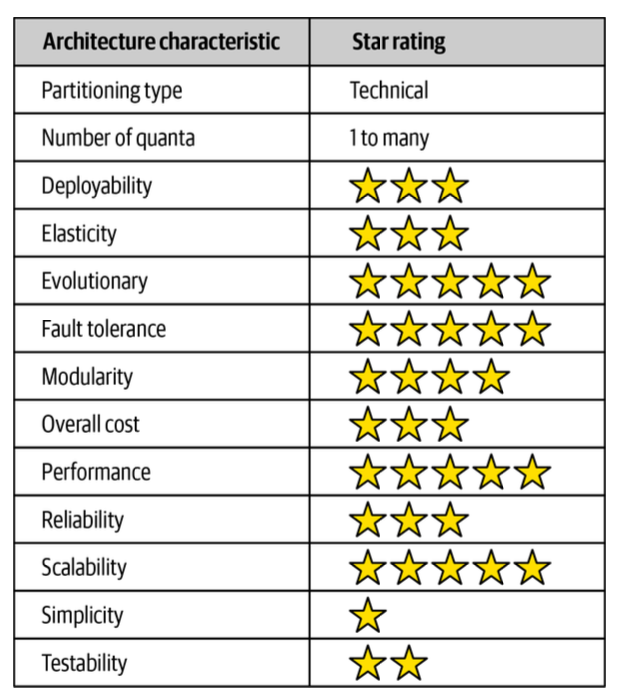
\includegraphics[width=\columnwidth]{Event_Driven.png} % Example image
	\caption{Event Driven Rating}
  \label{Event_Driven}
\end{figure}

Rating table found in Figure:\ref{Event_Driven} on page: \pageref{Event_Driven}. 

\subsection{Space based}

Space-based architecture gets its name from the concept of tuple space, 
the technique of using multiple parallel processors communicating through shared memory. 
High scalability, high elasticity, and high performance are achieved by removing the central 
database as a synchronous constraint in the system and instead leveraging replicated in-memory data grids. 
Application data is kept in- memory and replicated among all the active processing units. 
When a processing unit updates data, it asynchronously sends that data to the database, usually via 
messaging with persistent queues. Processing units start up and shut down dynamically as user load 
increases and decreases, thereby addressing variable scalability. Because there is no central database 
involved in the standard transactional processing of the application, 
the database bottleneck is removed, thus providing near- infinite scalability within the application.\\

\begin{figure}[h] % [h] forces the figure to be output where it is defined in the code (it suppresses floating)
	\centering
	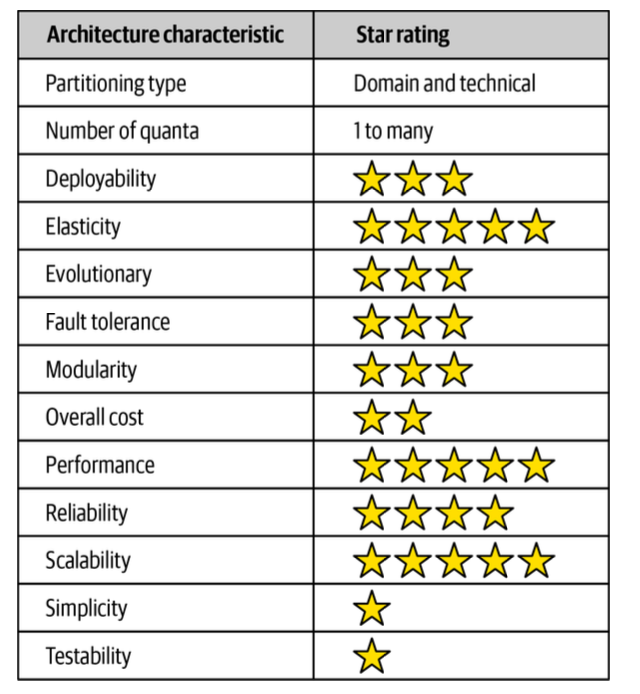
\includegraphics[width=\columnwidth]{Space_based.png} % Example image
	\caption{Space based Rating}
  \label{Space_based}
\end{figure}

Rating table found in Figure:\ref{Space_based} on page: \pageref{Space_based}.

\subsection{Microservices}

Microservices contain an API layer which guide request to each service which is a 
standalone program and database.
each service runs in its own process, 
which originally implied a physical computer but quickly evolved to virtual machines and containers.\\

\begin{figure}[h] % [h] forces the figure to be output where it is defined in the code (it suppresses floating)
	\centering
	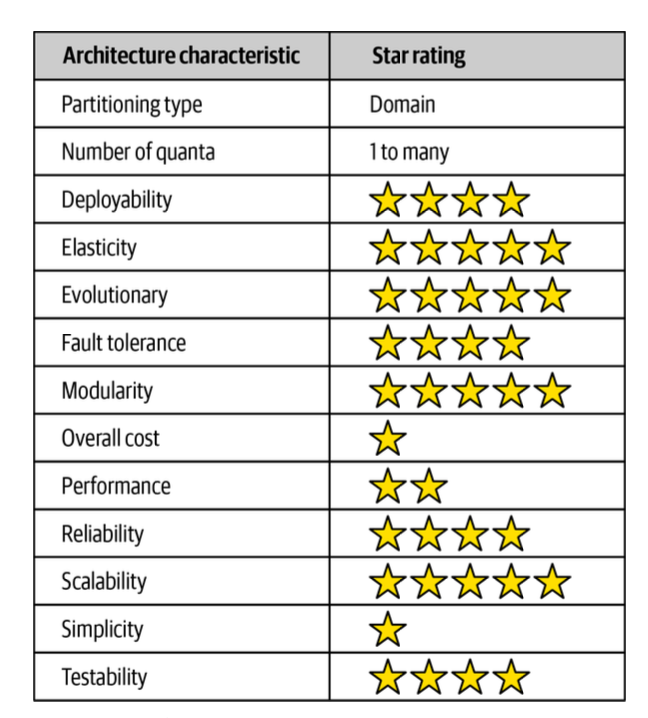
\includegraphics[width=\columnwidth]{Microservices.png} % Example image
	\caption{Microservices Rating}
  \label{Microservices}
\end{figure}

Rating table found in Figure:\ref{Microservices} on page: \pageref{Microservices}.

\section{Embedded software}

Issue of deep mingling between hardware elements and procedures.\\

\subsection{Hardware abstraction layers (HAL)}

Line between firmware and software is the HAL, the HAL handles the softwares need and access to the
the hardware. The software should not know anything about the hardware instead use concepts. Ie
BatteryLow NOT blinkLED.

The HAL also provides substitution points for the hardware to be used for testing to avoid the
target hardware bottleneck.

\textbf{Target Hardware Bottleneck:} Code can be only tested on the hardware.

\subsection{Processor abstraction layer (PAL)}

Separates the firmware into separate pieces to allow off hardware testing. Making the processor a 
plugin element. Can do a similar thing with an OS.

\section{Example}

\begin{enumerate}
  \item Determine actors and use cases
  \item Create component architecture
  \item Ensure dependency is appropriate for policy levels
  \item Determine deployment method of components
\end{enumerate}

\subsection{Use Cases}

Actors should be connected to use cases, abstract use cases can be used that connect other use
cases which add details to the abstract.

\subsection{Components}

Example pattern: View, presenter, interactor and controller are separated

\begin{itemize}
  \item Controller: Handle input
  \item Interactor: Process input into usable data
  \item Presenter: Format results
  \item Viewer: Display result
\end{itemize}

The vertical splits will be different actors/use cases.

\subsection{Types}

\subsubsection{Layered Architecture}

Boundaries drawn by technical difference, ie web, procedure and storage.\\

Doesn't have any link to the business or use case.

\subsubsection{Feature Architecture}

The boundaries are around features, but doesn't effectively separate technologies.

\subsubsection{Component Architecture}

Use boundaries and deployment method to separate technologies and use cases. A hybrid of the previous.

\subsection{Encapsulation}

If components have free access to each other, the architecture can be easily ignored. Utilizing
encapsulation allows the complier to ensure the architecture.

\section{Risk}

Use risk rating system which scores the impact of risk (1-3) and then the likelihood (1-3) and multiples for the
final risk score. This score should be marked against the supported characteristics, showing direction from
previous scores.

\pagebreak

\printbibliography[
heading=bibintoc,
title={Bibliography}
] %Prints the entire bibliography with the title "Whole bibliography"

%----------------------------------------------------------------------------------------
%	FIGURE EXAMPLE
%----------------------------------------------------------------------------------------

% \begin{figure}[h] % [h] forces the figure to be output where it is defined in the code (it suppresses floating)
% 	\centering
% 	\includegraphics[width=0.5\columnwidth]{IMAGE_NAME.jpg} % Example image
% 	\caption{European swallow.}
% \end{figure}

%----------------------------------------------------------------------------------------
% MATH EXAMPLES
%----------------------------------------------------------------------------------------

% \begin{align} 
% 	\label{eq:bayes}
% 	\begin{split}
% 		P(A|B) = \frac{P(B|A)P(A)}{P(B)}
% 	\end{split}					
% \end{align}

%----------------------------------------------------------------------------------------
%	LIST EXAMPLES
%----------------------------------------------------------------------------------------

% \begin{itemize}
% 	\item First item in a list 
% 		\begin{itemize}
% 		\item First item in a list 
% 			\begin{itemize}
% 			\item First item in a list 
% 			\item Second item in a list 
% 			\end{itemize}
% 		\item Second item in a list 
% 		\end{itemize}
% 	\item Second item in a list 
% \end{itemize}

%------------------------------------------------

% \subsection{Numbered List}

% \begin{enumerate}
% 	\item First item in a list 
% 	\item Second item in a list 
% 	\item Third item in a list
% \end{enumerate}

%----------------------------------------------------------------------------------------
%	TABLE EXAMPLE
%----------------------------------------------------------------------------------------

% \section{Interpreting a Table}

% \begin{table}[h] % [h] forces the table to be output where it is defined in the code (it suppresses floating)
% 	\centering % Centre the table
% 	\begin{tabular}{l l l}
% 		\toprule
% 		\textit{Per 50g} & \textbf{Pork} & \textbf{Soy} \\
% 		\midrule
% 		Energy & 760kJ & 538kJ\\
% 		Protein & 7.0g & 9.3g\\
% 		\bottomrule
% 	\end{tabular}
% 	\caption{Sausage nutrition.}
% \end{table}

%----------------------------------------------------------------------------------------
%	CODE LISTING EXAMPLE
%----------------------------------------------------------------------------------------

% \begin{lstlisting}[
% 	caption= Macro definition, % Caption above the listing
% 	language=python, % Use Julia functions/syntax highlighting
% 	frame=single, % Frame around the code listing
% 	showstringspaces=false, % Don't put marks in string spaces
% 	numbers=left, % Line numbers on left
% 	numberstyle=\large, % Line numbers styling
% 	]

% 	CODE

% \end{lstlisting}

%----------------------------------------------------------------------------------------
%	CODE LISTING FILE EXAMPLE
%----------------------------------------------------------------------------------------

% \lstinputlisting[
% 	caption=Luftballons Perl Script., % Caption above the listing
% 	label=lst:luftballons, % Label for referencing this listing
% 	language=Perl, % Use Perl functions/syntax highlighting
% 	frame=single, % Frame around the code listing
% 	showstringspaces=false, % Don't put marks in string spaces
% 	numbers=left, % Line numbers on left
% 	numberstyle=\tiny, % Line numbers styling
% 	]{luftballons.pl}

%----------------------------------------------------------------------------------------
%	BIB EXAMPLE
%----------------------------------------------------------------------------------------

% Using \texttt{biblatex} you can display a bibliography divided into sections, depending on citation type. 
% Let's cite! Einstein's journal paper \cite{einstein} and Dirac's book \cite{dirac} are physics-related items. 
% Next, \textit{The \LaTeX\ Companion} book \cite{latexcompanion}, Donald Knuth's website \cite{knuthwebsite}, \textit{The Comprehensive Tex Archive Network} (CTAN) \cite{ctan} are \LaTeX-related items; but the others, Donald Knuth's items, \cite{knuth-fa,knuth-acp} are dedicated to programming. 

% \medskip

% \printbibliography[
% heading=bibintoc,
% title={Whole bibliography}
% ] %Prints the entire bibliography with the title "Whole bibliography"

% %Filters bibliography
% \printbibliography[heading=subbibintoc,type=article,title={Articles only}]
% \printbibliography[type=book,title={Books only}]

% \printbibliography[keyword={physics},title={Physics-related only}]
% \printbibliography[keyword={latex},title={\LaTeX-related only}]

\end{document}